% !Mode:: "TeX:UTF-8"
\newcommand{\us}{\_}

\chapter{方法设计与实现}

\section{方法概述(Pipeline)}

该对象操纵交互系统的方法流程可以用一个有限状态机来表示。

\begin{figure}[b!]
    \centering
    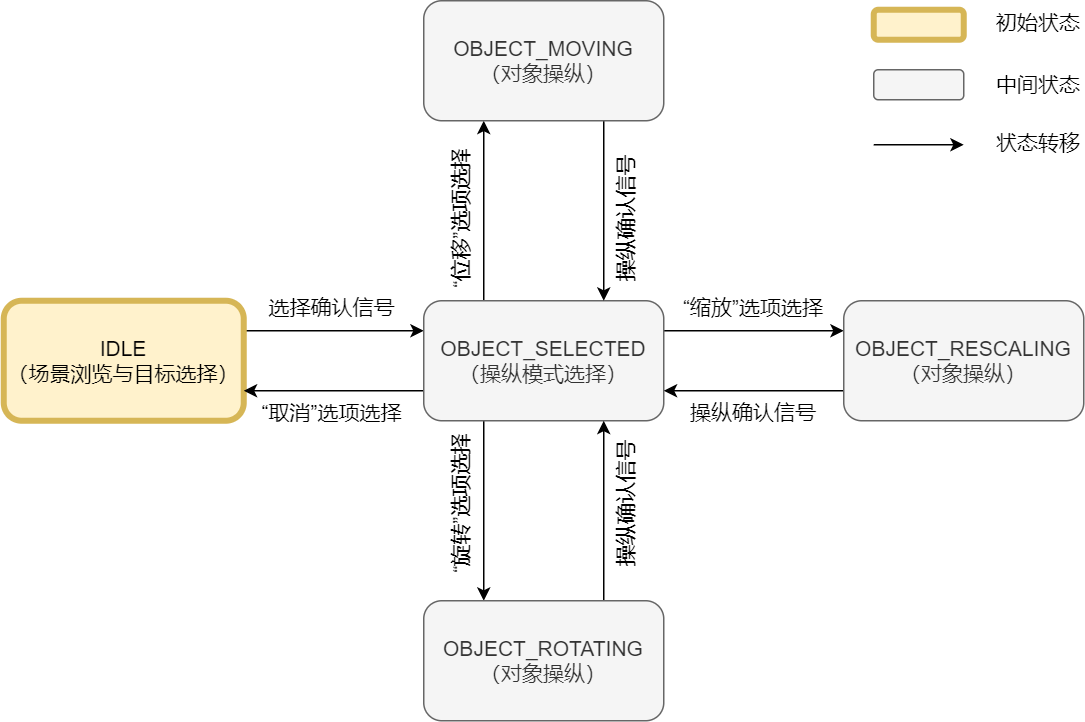
\includegraphics[width=.85\textwidth]{figure/system_state_machine.png}
    \caption{交互系统状态机}
    \label{fig-3-1}
\end{figure}

{\bf 场景浏览与目标选择}:对应状态IDLE。在进行目标选择时,用户先以通过头部向前射线指向目标操纵对象,之后以快速两次眨眼作为确认信号选择该对象,该选择和确认方法的优势由Yuan Yuan Qian团队在2017年作过探讨\upcite{yuanyuan2017}。接收到选择确认信号后,进入下一状态;

{\bf 操纵模式选择}:对应状态OBJECT\us SELECTED。生成一个“四叶草”模式选择菜单,用户可以通过凝视某一选项以进入对应的操纵模式,用户也可以通过凝视“返回”选项以退回到1(详见\autoref{Clover});

{\bf 对象操纵}:对应状态OBJECT\us MOVING、OBJECT\us ROTATING或OBJECT\us RESCALING。我们提出的操纵系统支持六自由度(6DOF)操纵。在不同的对象操纵模式下,用户可以对物体进行三自由度位移、二自由度旋转和一自由度缩放(详见\autoref{Manipulation});

{\bf 确认操纵结果}:对应状态转移条件“操纵确认信号”。通过快速两次眨眼作为确认信号以确认当前操纵状态,回到OBJECT\us SELECETD。

\section{场景浏览与目标选择}

\section{“四叶草”模式选择菜单}\label{Clover}

\subsection{设计理念}

我们在交互系统设计阶段考虑到大多数实际的完整操纵流程往往不仅包含一个特定操纵模式的选择,还会包含多种操纵模式之间的切换。然而,当前的基于凝视和眼动的交互方法并没有考虑便捷的模式切换;在这些方法中,如果用户需要在一次操纵结束后切换到下一种操纵模式,则需要退回到最初态重新进行一遍从选择到操纵到流程,引入大量冗杂操纵和效率浪费。所以基于此考虑,我们设计了一个“四叶草”模式选择菜单。

我们希望“四叶草”模式选择菜单可以让用户简便地用凝视动作来选择进入或者切换到某种交互状态。

菜单在四个方向提供了四个的选项,分别为位移、旋转、缩放和取消;用户可以通过看向相应的方向来选择对应的选项。当用户选择时,界面上会显示一个选择确认进度盘,用户可以在进度盘进度未满之前通过使视线复位来取消选择;当进度盘进度满后,用户立即转移至对应的状态。

\subsection{菜单说明}

\subsection{线性优化}

\section{对象操纵}\label{Manipulation}
